\section{Einleitung}

Diese Dokumentation gibt einen Überblick über das Semesterprojekt im Modul Software-Engineering des Medieninformatik-Masterstudienganges.
Ziel des Projekts ist es, eine anwendungsspezifische Sprache (domain-specific language) zu entwicklen und anhand dieser Code einer höheren Programmiersprache zu generieren.
Der generierte Code soll hierbei eine zu implementierende Anwendung komplettieren und somit der Umgang mit anwendungsspezifischen Sprachen sowie der Codegenerierung praxisnah geübt und gefestigt werden.

Die Anforderung wird anhand eines Spiels und eines Levelgenerators umgesetzt.
Der Levelgenerator übernimmt hierbei die Verarbeitung der anwedungsspezifischen Sprache.

\subsection{Spielidee}

Es soll ein 2D Spiel in Top-Down Perspektive entwickelt werden.
Der Spielziel ist es, ein sich ständig leerendes Bier rechtzeitig durch den Besuch eines Spätis wieder aufzufüllen und bis zum Ende einer vorher definierten Zeit das Bier nicht leer werden zu lassen.
Dazu bewegt der Spieler sich in einer blockbasierten Welt.
Diese enthält sowohl Spätis zum nachfüllen des Bieres, als auch Gegner welche den Füllstand des Bieres oder die Geschwindigkeit des Spieler reduzieren können.
In Abbildung \ref{fig:einleitung:screenshot} wird eine typische Szene des Spiels gezeigt.

\begin{figure}[]
\centering
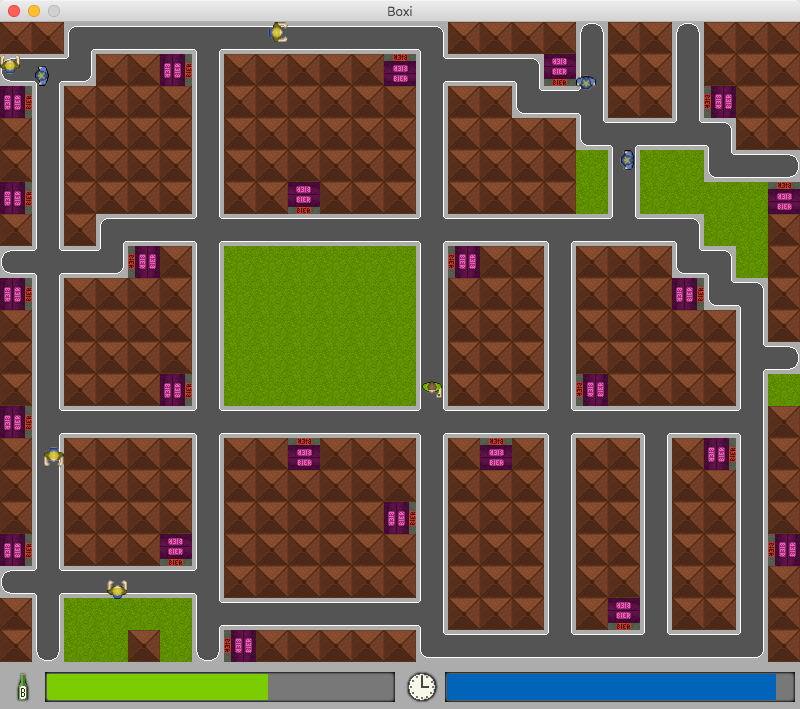
\includegraphics[width=3in]{img/02_screenshot.png}
\caption{Screenshot des Spiels}
\label{fig:einleitung:screenshot}
\end{figure}


\subsection{Zweck der Codegenerierung}
\todo{stubs}
- Anordnung der Blöcke (mögliche Blöcke werden in ... beschrieben)
- Startpunkt des Spielers
- Startpunkt der Gegner
- Angriffswerte der Gegner
- Initiale Werte des Spielers